\PassOptionsToPackage{unicode}{hyperref}
\documentclass[aspectratio=1610, professionalfonts, 9pt]{beamer}

\usefonttheme[onlymath]{serif}
\usetheme[showtotalframes]{tudo}


\usepackage{polyglossia}
\setmainlanguage{english}


\usepackage[
  backend=biber,   % use modern biber backend
  autolang=hyphen, % load hyphenation rules for if language of bibentry is not
                   % german, has to be loaded with \setotherlanguages
                   % in the references.bib use langid={en} for english sources
]{biblatex}
\addbibresource{references.bib}  % die Bibliographie einbinden
\DefineBibliographyStrings{german}{andothers = {{et\,al\adddot}}}


% Mathematik
\usepackage{multicol}
\usepackage{graphicx}
\usepackage{amssymb}
\usepackage{amsmath}
\usepackage{xparse}
\usepackage{braket}
\usepackage{units}
\usepackage[locale=DE,separate-uncertainty=true,per-mode=reciprocal,output-decimal-marker={,},]{siunitx}
\usepackage[section]{placeins}
\usepackage{pdflscape}
\usepackage{expl3}
\usepackage{bookmark}
%Komma als Dezimaltrenner in der mathe Umgebung, um in Umgebungen wie [0, 2] ein Leerzeichen nach dem Komma zu erhalten einfach eins setzen
\usepackage{icomma}
\usepackage{cancel}
\usepackage{hyperref}
\usepackage{bookmark}
\usepackage{subfigure}

%%%%%%%%%%%%%%%%%%%%%%%%%%%%%%%%%%%%%%%%%%%%%%%%%%%%%%%%%%%%%%%%%%%%%%%%%%%%%%%%
%%%%%-------------Hier Titel/Autor/Grafik/Lehrstuhl eintragen--------------%%%%%
%%%%%%%%%%%%%%%%%%%%%%%%%%%%%%%%%%%%%%%%%%%%%%%%%%%%%%%%%%%%%%%%%%%%%%%%%%%%%%%%

%Titel:
\title{Optimimizing the Energy Reconstruction for CTAs analysis by combining predictions of different Telescope IDs}
%Autor
\author[L.~Möllerherm]{Lars Möllerherm}
%Lehrstuhl/Fakultät
\institute[Experimentelle Physik Vb]{Experimentelle Physik Vb \\  Fakultät Physik}

\begin{document}

\maketitle

\section{Data}
  \begin{frame}
    \frametitle{Steps done for a better Reconstruction}
    \begin{itemize}
      \item data: Monte Carlo data (PROD3(B)) \- pointlike gamma (?? events).

      \item Used attributes for the RF:
      \begin{itemize}
        \item length
        \item width
        \item skewness
        \item kurtosis
        \item intensity and total intensity
        \item scaled width an length
        \item num triggered telescopes(lst; mst; sst)
        \item telescope type id
      \end{itemize}

      \item steps:
      \begin{itemize}
        \item taking scaled width and length  \cite[104]{HESS}: $SW =\frac{w(q,p)-\langle w(q,p) \rangle}{\sigma_w(q,p)}$  $SL = \frac{l(q,p)-\langle l(q,p) \rangle}{\sigma_l(q,p)}$
        \item taking an weighted mean(weight: sensitivity [$2 = \text{full sensitivity}$; $1 = \text{required energy range}$; $0.1 = \text{out of energy range}$]).
        \item taking the weighted(sensitivity) mean as a new attribute for another RF.
      \end{itemize}
    \end{itemize}

  \end{frame}


\section{Performance}
  \begin{frame}{Performance with and without weighted mean}
      \begin{columns}
        \begin{column}{0.5\textwidth}
          \begin{figure}
            \centering
            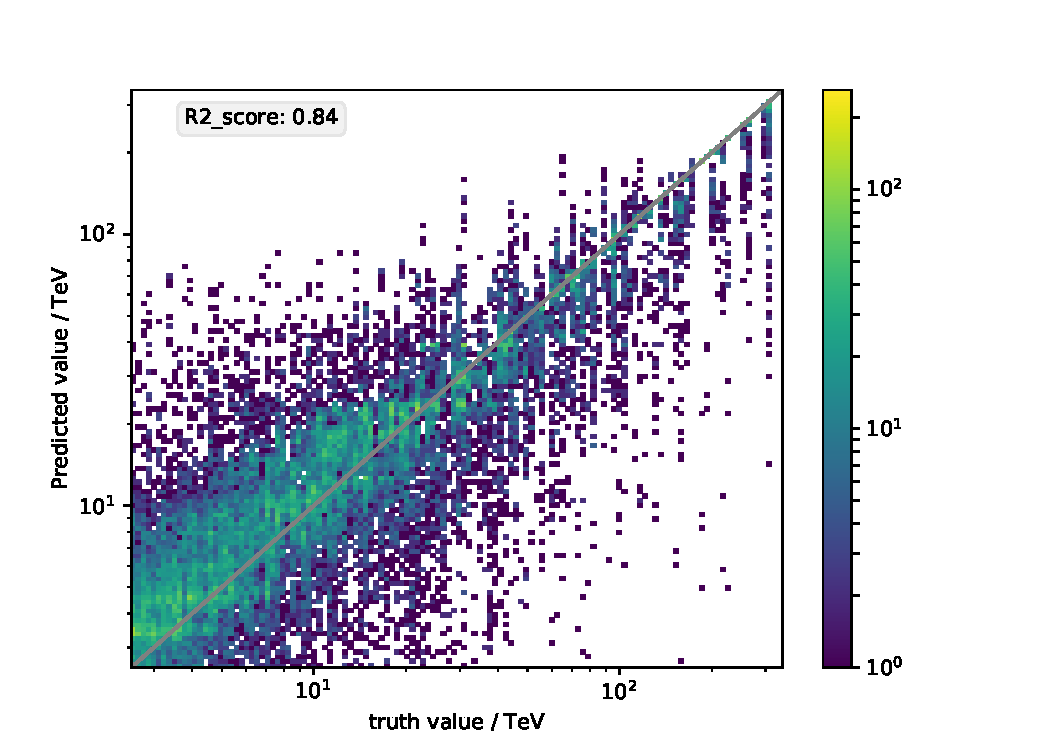
\includegraphics[width=\textwidth]{Plots/RF_MSV.pdf}
            \caption{Energy reconstriction by a Random Forest Regressor by the use of the MSV.}
          \end{figure}
        \end{column}
        \begin{column}{0.5\textwidth}
          \begin{figure}
            \centering
            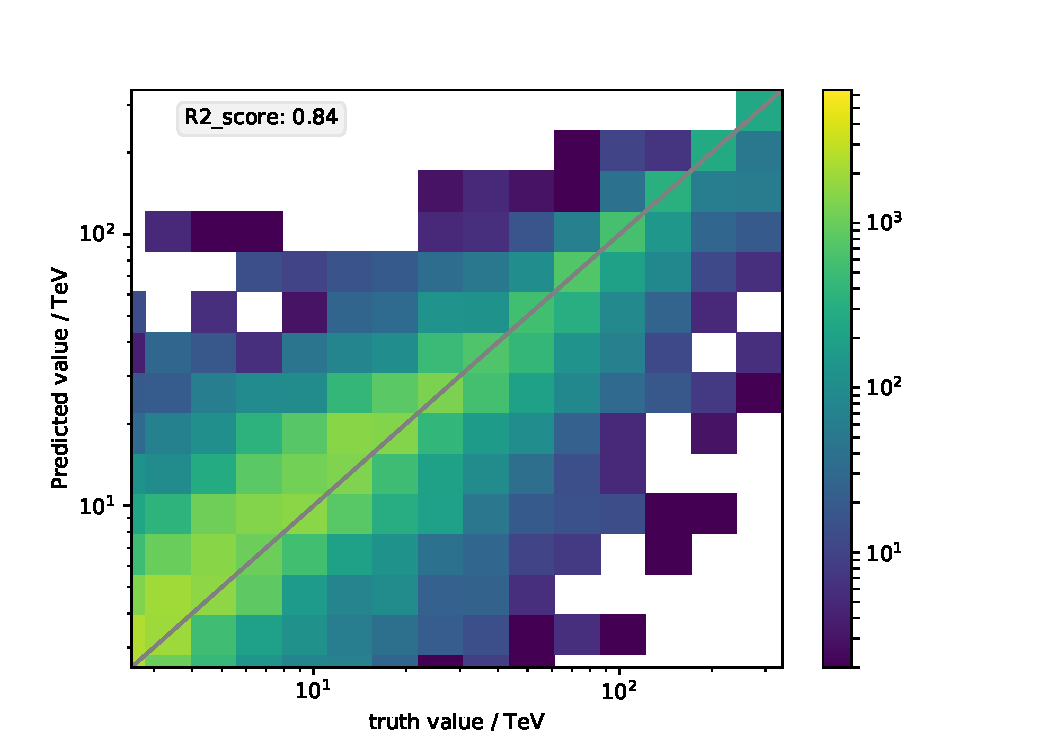
\includegraphics[width=\textwidth]{Plots/RF_MSV_wI_mean.pdf}
            \caption{Building the average over the telescopes which have seen the same event, by using the intensity as a weight.}
          \end{figure}
        \end{column}
      \end{columns}
  \end{frame}

  \begin{frame}
    \begin{columns}
        \begin{column}{0.5\textwidth}
          \begin{figure}
            \centering
            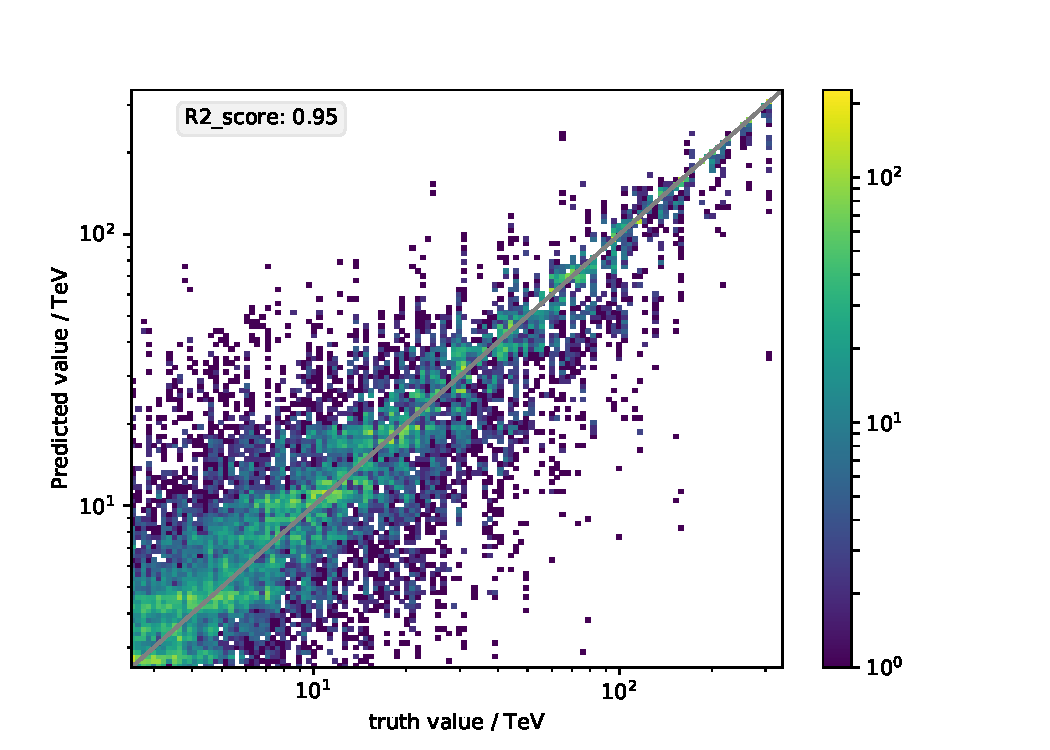
\includegraphics[width=\textwidth]{Plots/RF_MSV_encaps.pdf}
            \caption{Taking the weighted mean as a new attribute for a second Random Forest Regressor.}
          \end{figure}
        \end{column}
        \begin{column}{0.5\textwidth}
          Attributes of the second RandomForest:
          \begin{itemize}
            \item weighted mean(sensitivity) of prediction
            \item mean(std, max, min) of the prediction of all LST(MST, SST)
            \item mean(std) of scaled values
          \end{itemize}
        \end{column}
    \end{columns}

  \end{frame}

  \begin{frame}
    \begin{columns}
      \begin{column}{0.5\textwidth}
        \begin{figure}
          \centering
          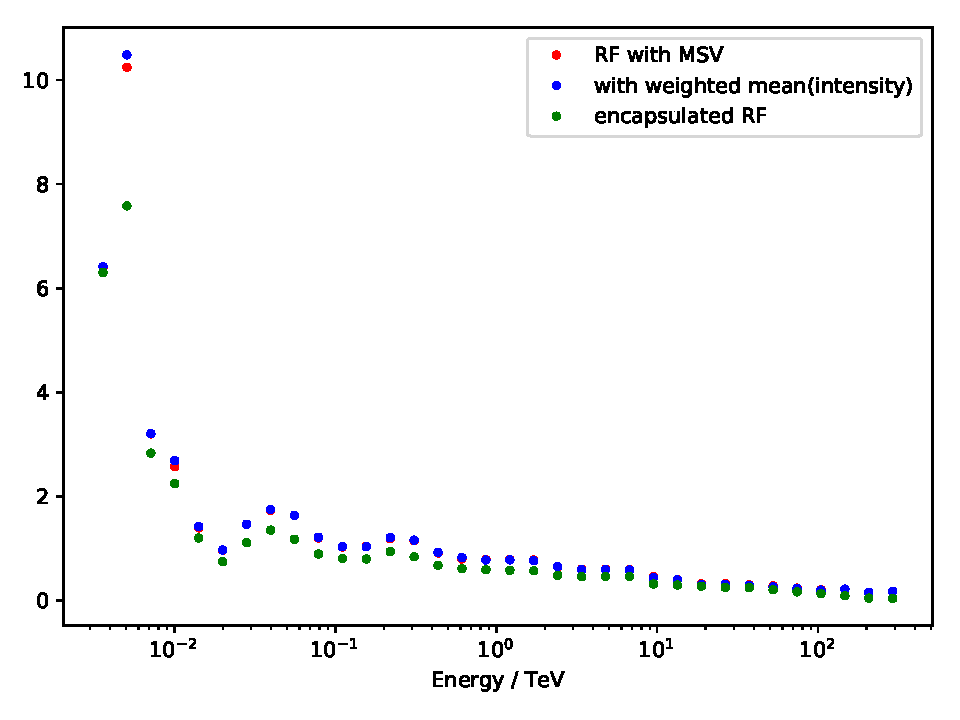
\includegraphics[width=\textwidth]{Plots/RF_MSV_rel_mean.pdf}
          \caption{Bias in every bin for all three predictions.}
        \end{figure}
      \end{column}
      \begin{column}{0.5\textwidth}
        \begin{figure}
          \centering
          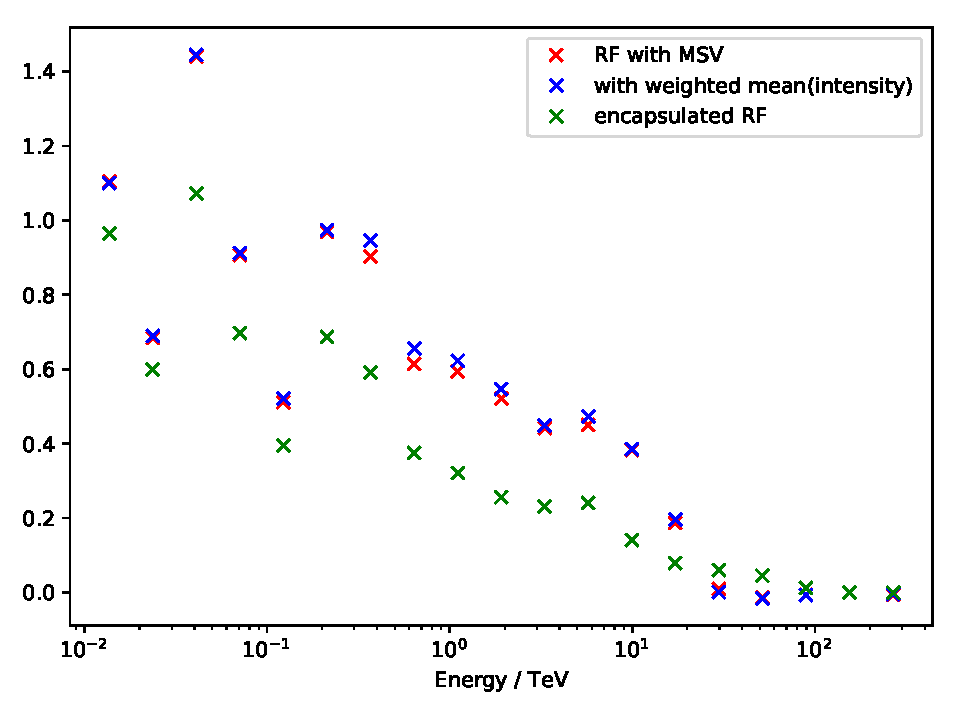
\includegraphics[width=\textwidth]{Plots/RF_MSV_rel_std.pdf}
          \caption{$68.3\,\%$-Quantil of the relativ error in every bin for all three predictions.}
        \end{figure}
      \end{column}
    \end{columns}
  \end{frame}

\section{Attributes}
  \begin{frame}{Importance of the attributes}
    \begin{columns}
      \begin{column}{0.5\textwidth}
        \begin{figure}
          \centering
          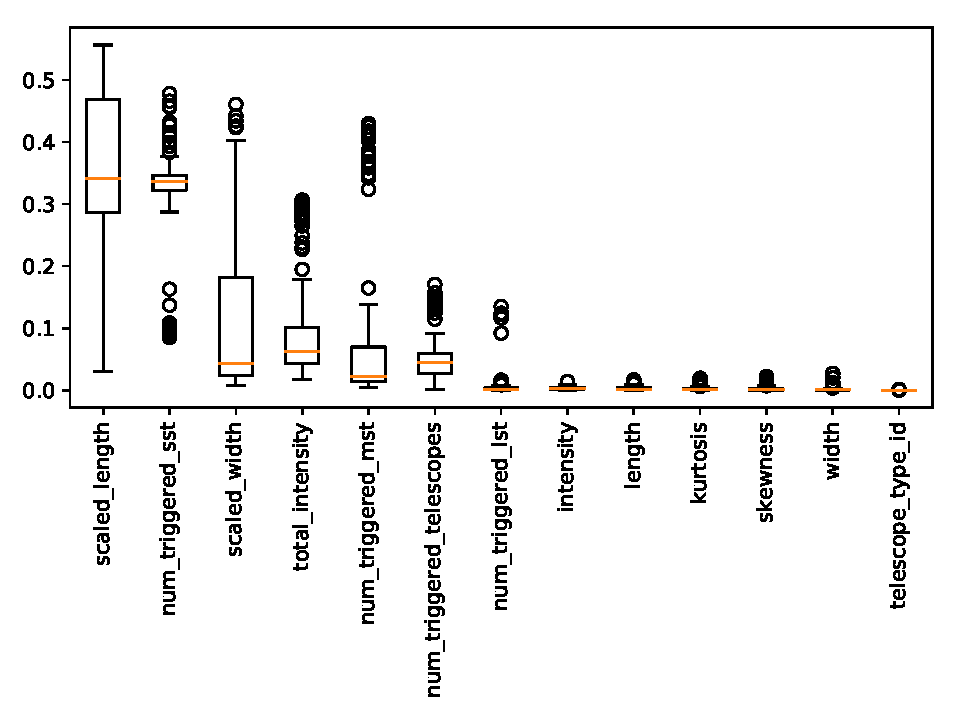
\includegraphics[width=\textwidth]{Plots/feautureimportance_boxplot.pdf}
          \caption{Importance of the used attributes bei the first prediction.}
        \end{figure}
      \end{column}
      \begin{column}{0.5\textwidth}
        \begin{figure}
          \centering
          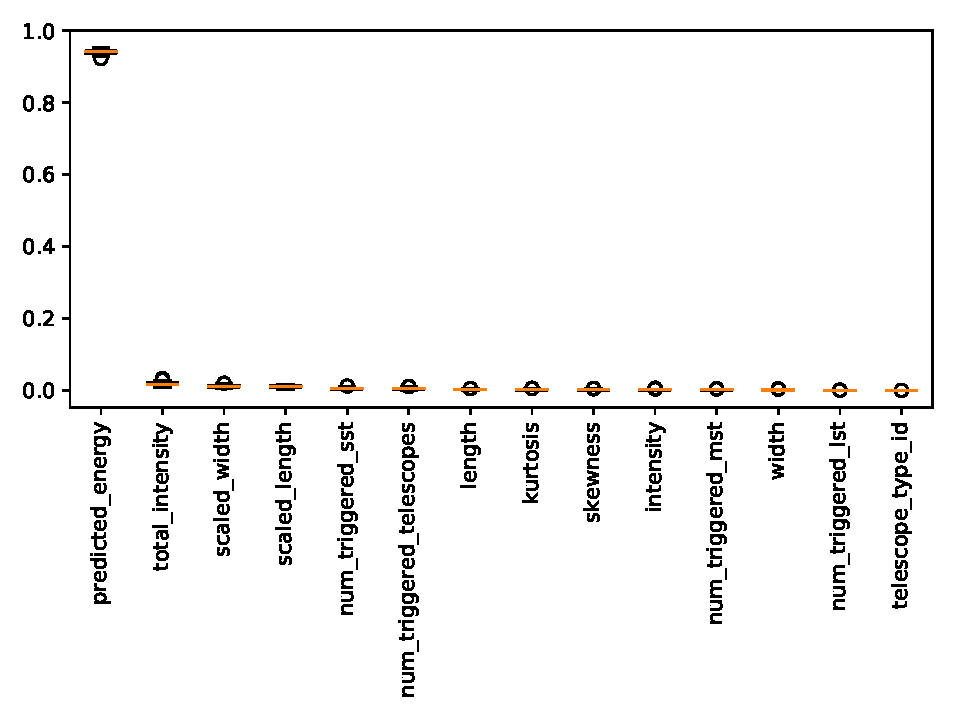
\includegraphics[width=\textwidth]{Plots/feautureimportance_boxplot_secondForest.pdf}
          \caption{Importance of the used attributes bei the second prediction.}
        \end{figure}
      \end{column}
    \end{columns}
  \end{frame}
\section{References}
  \printbibliography
\end{document}
